\chapter{Introduction à théorie de la relativité restreinte}
	

	\section{Principe de relativité et propagation du champ}
		Pour décrire les phénomènes de la nature, nous avons besoin de systèmes de références, c'est-à-dire d'objets physiques (parfois imaginaires) que l'on suppose fixes et par rapport auxquels nous mesurons la dynamique d'autres objets physiques. Mathématiquement, ces objets physiques sont conceptualisés par des systèmes de coordonnées dans lesquels la dynamique des objets physiques est décrite. La théorie mécanique selon Newton postule l'existence de certains systèmes de références dans lesquels les objets dont la résultante des actions qu'ils subissent est nulle ont un mouvement soit immobile, soit rectiligne uniforme (se déplaçant en ligne droite à vitesse constante). Ceci constitue la première loi de Newton, qui est très importante. Une conséquence des deux premières lois de Newton bien connue est que si un référentiel est en translation rectiligne uniforme par rapport à un référentiel galiléen, alors ce référentiel est aussi galiléen. De là, il suit que ce second référentiel peut être choisi comme système de référence, et c'est alors l'autre référentiel, initialement immobile, qui sera vu en mouvement par rapport au second référentiel. Ainsi, et cela est (normalement) enseigné depuis le collège, le mouvement des corps n'a de sens que s'il est défini par rapport à un système de référence. Continuons notre réflexion : l'affirmation "le Soleil tourne autour de la Terre" n'est ni vraie, ni fausse, puisque le système de référence par rapport auquel le mouvement "tourne" n'a pas été précisé. Pour ceux qui pensent que cette affirmation est fausse : de mon point de vue, je vois, chaque jour, depuis l'aube au crépuscule, en passant par midi, le Soleil tourner autour de moi. Dans le système de référence lié à mon bureau, le Soleil tourne autour de la Terre. Pour ceux qui pensent que cette affirmation est vraie : si on pouvait placer un observatoire sur le Soleil, on y observerait la Terre tourner autour.

		Ce principe a d'abord été énoncé par Galilée avant d'être formalisé et unifié par les lois de Newton. Pour passer d'un référentiel galiléen à un autre selon la théorie de Newton, il faut effectuer une transformation galiléenne, décrite formellement par la transformation suivante\footnote{Les vecteurs spatiaux sont notés en gras.}:
		\begin{eqnarray}
			t'(t,\bm{x})&=&t \\
			\bm{x}'(t,\bm{x})&=&\bm{x}+\bm{C}_0+\bm{v}t
		\end{eqnarray}
		où $\bm{C}_0$ et $\bm{v}$ sont des vecteurs constants. Les lois de la physiques sont invariantes par une telle transformation : si l'on exprime les lois de la physique dans l'un ou dans l'autre des référentiels galiléens, on trouvera les mêmes équations. La théorie Newtonienne, qui postule un temps universel séparé de l'espace, fonctionnait redoutablement bien jusqu'à la fin du XIXème siècle\ldots tant que l'on n'essayait pas d'y inclure l'électromagnétisme. En effet, les équations de Maxwell, qui elles aussi sont terriblement efficaces pour décrire les phénomènes électriques, ne sont pas invariantes par une transformation galiléenne ! Au début du XXème siècle, cela fait déjà deux cents ans que la théorie de la mécanique de Newton explique moult phénomènes avec une précision démoniaque ; il est donc hors de question de la remettre en cause, c'est à la théorie électromagnétique, qui n'a qu'une trentaine d'années, de se plier à son aînée. Un autre fait important est que les physiciens de l'époque postulaient l'existence d'un éther, substance dans laquelle se déplaçaient les ondes électromagnétiques. Cet éther était supposé être absolument immobile, ce qui supposait la prévalence de certains référentiels sur d'autres. 

		C'est alors qu'un jeune moustachu, sans poste de professeur ou chercheur dans aucun laboratoire ni université, qui travaillait à l'office des brevets de Berne, eut des considérations fortement esthétiques sur la théorie. Albert Einstein tenait à cette invariance des lois de la physique par changements de référentiels, et décida d'abandonner l'Ether, donnant ainsi naissance à la théorie des champs. De plus, le jeune Albert (qui avait 26 ans en 1905) décida d'abandonner l'idée de temps absolu, pour lui préférer l'idée qu'il existait autant de temps propres que d'observateurs (réels ou fictifs).

		Le principe de relativité affirme donc que les lois de la nature sont les mêmes dans tous les référentiels galiléens. Cependant, les transformations de Galilée ne semblent pas permettre de passer correctement d'un référentiel galiléen à un autre puisque les lois de l'électromagnétisme ne sont plus valables. Einstein fut le premier à oser remettre en cause les lois de Newton. Une façon simple de comprendre ceci est ce qui suit.

		La gravitation de Newton induit l'instantanéité des propagations du champ de gravitation. Selon la loi de gravitation de Newton, si le Soleil disparaît, la Terre cessera immédiatement de tourner et continuera sa vie dans une trajectoire rectiligne uniforme (sans tenir compte des autres planètes, pour simplifier). Or, comme nous le verrons plus bas, la notion de synchronisation ne peut être absolue, donc la notion de temps absolu, qui inclut qu'une synchronisation absolue de toutes les horloges est possible, doit être abandonnée. L'expérience montre que lorsque deux corps interagissent, si l'un subit des modifications, l'autre n'en sera affecté qu'au bout d'un certain temps. En divisant la distance séparant les deux corps par le temps de réaction dont nous venons de parler, une notion de "vitesse de propagation des interactions" émerge. Le second postulat fondamental de la théorie de l'espace-temps (nommée classiquement "relativité restreinte") est que la vitesse de propagation des interactions admet un maximum. Si nous admettons que ces postulats sont vrais, nous pouvons d'emblée montrer qu'aucun corps ne peut se déplacer plus vite que cette vitesse maximale. En effet, si c'était le cas, ce corps pourrait être utilisé pour véhiculer une interaction avec une vitesse plus grande que la vitesse maximale de propagation de ces interactions. 

		Cette vitesse maximale de propagation des interactions est souvent nommée "vitesse de propagation du signal". Au risque de tuer le suspense, cette vitesse maximale de propagation des interactions est la vitesse de la lumière dans le vide, et sa valeur numérique est exactement:
		\begin{equation}
			c=299\, 792\, 458\, \mathrm{m}/\mathrm{s}.
		\end{equation}
		Depuis 1983, la vitesse de la lumière dans le vide est en effet exacte, par définition du mètre, celui-ci étant défini comme la longueur du trajet parcouru dans le vide par la lumière pendant une durée de 1/299 792 458 seconde. 

		En raison de la grande valeur numérique de cette constante, on peut comprendre que pour des corps se déplaçant lentement par rapport à cette vitesse, la loi de gravitation de Newton, ainsi que le caractère absolu du temps, soient de bonnes approximations. Lorsque l'on suppose que les deux postulats précédents sont vrais, le cadre théorique utilisé est nommé \emph{mécanique relativiste}. Lorsque l'on suppose que les vitesses d'interactions sont infinies et que le temps est absolu, le cadre théorique est nommé \emph{mécanique de Newton}. Il est possible de passer formellement de la mécanique relativiste à la mécanique de Newton en posant $c\rightarrow\infty$ dans les équations\footnote{Nous évitons les termes souvent employés de "mécanique classique", qui peuvent porter à confusion. En effet, "mécanique classique" peut signifier "mécanique non quantique" ou "mécanique non relativiste", mais il est possible de formuler des théories relativistes non quantiques, ainsi que des théories quantiques non relativistes, et là, tout le monde est perdu. Nous nous interdisons ainsi les termes "mécanique classique" pour plus de clarté.}. 

		En mécanique de Newton, le caractère absolu du temps, \emph{i.e.} son indépendance des systèmes de références, implique que si un observateur attaché à un référentiel observe deux phénomènes simultanés, alors tout observateur dans tout autre référentiel observera également ces deux phénomènes comme simultanés. Or il est facile de s'assurer que le concept de temps absolu est en contradiction avec le principe d'universalité de la vitesse de propagation des phénomènes. En effet, la mécanique de Newton, basée sur le concept de temps absolu, se base sur les transformations de Galilée de composition vectorielle des vitesses. Or, comme cette loi est universelle, elle devrait être vraie pour la vitesse de propagation des informations, et impliquerait qu'il serait possible de dépasser ce maximum, ou encore que cette vitesse maximale dépendrait du référentiel. Mais l'expérience montre que c'est le principe de relativité qui est vrai. En effet, les expériences de Michelson de la fin du XIXème siècle ont montré que la vitesse de propagation de la lumière était indépendante de la direction de propagation dans un référentiel en mouvement par rapport à l'objet qui émet de la lumière. 

		\begin{figure}
			\centering
			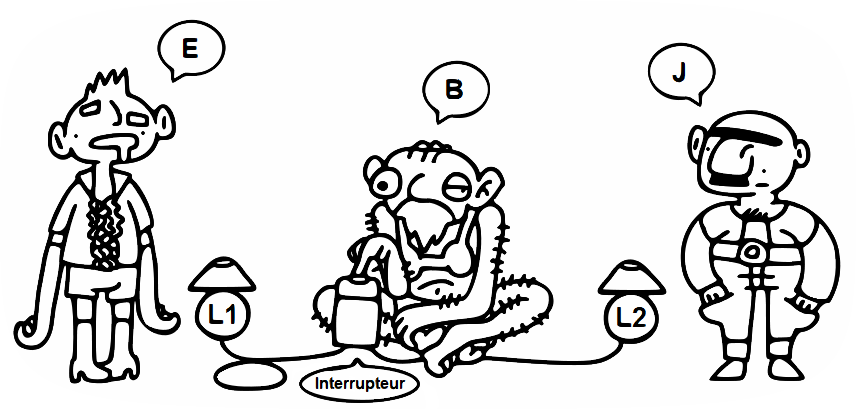
\includegraphics[scale=0.5]{../cours/bb_by_eurydrama-d9uaffl.png}
			\caption{Dispositif expérimental mettant en évidence le caractère relatif de la simultanéité.}
			\label{pluthaar}
		\end{figure}

		Pour être plus clairs, imaginons un exemple simple. Soit trois observateurs $B=$Bernard, $J=$Jean-Jacques, $E=$Eudes-Kévin, situés selon la figure \ref{pluthaar}. Les deux lampes $L_1$ et $L_2$ sont disposées à égales distances de Bernard. À $t=0$, Bernard appuie sur un interrupteur. Le signal électrique se propage le long des deux fils, et les deux lampes s'allument. Le signal lumineux met $\Delta t_1=L_1B/c=L_2B/c$ à parvenir à Bernard, celui-ci voit donc les deux lampes s'allumer en même temps. Cependant, pour Jean-Jacques, les choses sont différentes. En effet, comme $L_1J>L_2J$, ce gars-là verra la lampe $L_2$ s'allumer avant la lampe $L_1$. La situation est inverse pour Eudes-Kévin. Ainsi, la simultanéité pour un observateur n'implique pas la simultanéité pour tous les observateurs en théorie relativiste. Notons à ce stade que le principe de causalité n'est pas remis en question. En effet, l'allumage de la lampe $L_1$ n'est pas la cause de l'allumage de la lampe $L_2$, et réciproquement ; ces événements peuvent donc apparaître dans un ordre quelconque selon le référentiel. En revanche, que ce soit pour Jean-Jacques ou Eudes-Kévin, les deux verront Bernard appuyer sur l'interrupteur toujours avant l'allumage de l'une ou de l'autre lampe, à deux conditions : la vitesse de propagation du courant électrique est plus faible que la vitesse de la lumière, et les deux observateurs (Jean-Jacques et Eudes-Kévin) se déplacent eux-mêmes plus lentement que la lumière\footnote{Dans le cas où l'un des trois phénomènes est aussi rapide que la vitesse de la lumière, il peut au mieux y avoir simultanéité apparente.}. Malgré le caractère relatif du temps, mettons définitivement fin aux faux espoirs : la causalité est absolue dans la théorie relativiste de l'espace-temps. Cela sera aussi vrai en relativité générale. Il est absolument impossible de modifier son passé en théorie relativiste. Enfin, notons que la causalité absolue est une conséquence du caractère fini du maximum de la vitesse des propagations.

		Une autre conséquence du principe de relativité est que les solides indéformables n'existent pas. En effet, si c'était le cas, le choc d'un autre solide sur un solide donné impliquerait un mouvement d'ensemble comme conséquence d'un choc en un point de contact. Ainsi, un autre point du solide indéformable, éloigné du point de contact, serait animé d'un mouvement instantanément après le choc, ce qui est contraire avec la vitesse de propagation finie des informations. Les points du solide éloignés du point de contact doivent "attendre" que l'information de la perturbation du point de contact arrive jusqu'à eux, et cette information ne peut se transmettre instantanément.

		Énonçons une bonne fois pour toute le principe de relativité d'Einstein :

		\hspace{-0.5cm}\fbox{\parbox{\textwidth}{Les lois de la nature sont les mêmes dans tous les référentiels inertiels. De plus, la propagation des signaux et des interactions entre les corps admet une vitesse maximale universelle qui est la même dans tous les référentiels inertiels.}}

		Discutons un peu des conséquences de ce principe. Une autre façon de l'énoncer est de dire que le mouvement\footnote{Sous-entendu rectiligne uniforme.} est comme rien.  Toutes les expériences physiques donneront strictement les mêmes résultats dans tous les référentiels galiléens. Si vous changez d'un référentiel à un autre, la vitesse de la lumière sera toujours "infiniment" éloignée de vous. En effet, si vous accélérez pour gagner, mettons, $100\mathrm{km}/\mathrm{s}$, vous ne faites que passer d'un référentiel inertiel à un autre. Une fois que vous vous situez dans ce second référentiel inertiel, vous pouvez alors tout remettre à zéro et annuler votre vitesse. Du point de vue d'un observateur, la lumière est donc perpétuellement inateignable, quels que soient les efforts fournis. Un deuxième observateur qui voit le premier accélérer perpétuellement, ne le verra jamais dépasser la vitesse de la lumière ; il peut au mieux l'observer s'en approcher asymptotiquement, comme nous le montrerons bientôt. Le principe de relativité est une démocratisation des référentiels inertiels : ceux-ci se valent tous.

		Il suit aussi que la constante $c$ est une constante universelle de la physique. La vitesse de la lumière n'est pas le résultat de calculs, elle est profondément ancrée dans les postulats même de la théorie. Nous verrons également abondamment que les seuls protocoles expérimentaux fiables se fondent sur la propagation de la lumière. Les seules mesures fondamentales de distances sont en fait des mesures de temps de propagation de la lumière, que nous multiplions par $c$ pour obtenir des distances.

		Pour finir ce paragraphe d'introduction, discutons de la notion de théorie du champ. Deux objets ne peuvent interagir que via un champ d'interaction dont les modifications ne peuvent se propager que localement de proche en proche, et la vitesse de cette propagation est universellement (dans tous les référentiels inertiels) limitée par la vitesse de la lumière. Comme nous le verrons, le champ lui-même est un objet physique. Conceptuellement, il faut donc comprendre que deux objets qui interagissent constituent en réalité trois objets physiques : les deux objets dont on souhaite déterminer théoriquement la dynamique, et le champ d'interaction entre ces deux objets. En théorie du champ, lorsqu'on place deux objets ensemble, on ne peut les étudier correctement qu'en étudiant trois objets.

	\section{Description mathématique de l'espace-temps : première approche naïve} 

		Nous donnons ici une première appréhension de l'espace-temps, en développant le minimum de formalisme mathématique pour rester rigoureux. Les armes mathématiques de destruction massive qui permettent de tuer les problèmes en un battement de cils seront développées plus tard.

		Si nous voulons décrire les objets de la nature, nous ne pouvons plus distinguer l'espace et le temps. Chaque événement de l'espace-temps sera donc caractérisé par une position dans l'espace, et une date, toutes ces quantitées étant observées par un observateur lié à un système de référence. Comme l'espace est à trois dimensions, il faut trois coordonnées ; en repérage cartésien il est usuel de choisir $x,y,z$. Essayons de traduire cela en terme mathématique. Pour un observateur $\mathscr{O}$ placé au centre d'un repère, chaque événement est repéré par quatre coordonnées d'espace-temps : $(ct,x,y,z)\equiv (x^0,x^1,x^2,x^3)$. La coordonnée temporelle a été multipliée par $c$ pour avoir les mêmes dimensions que les coordonnées spatiales. Puisque la théorie de Newton est inefficace, nous devons traîter l'espace et le temps $\emph{a priori}$ de la même façon. Ainsi, les objets de la nature évoluent dans un espace à quatre dimension que nous nommons espace-temps. 

		Essayons d'exprimer le principe de relativité. Soient deux observateurs $\mathscr{O}$ et $\mathscr{O}'$ liés à deux référentiels $\mathscr{R}$ et $\mathscr{R}'$, tous deux inertiels, dans lesquels on peut mesurer des événements à des dates $t$ et $t'$, localisées dans l'espace par les coordonnées $x,y,z$ et $x',y',z'$. Faisons coincider les axes $x$ et $x'$ et faisons de telle sorte que les axes $y$ et $y'$ soient parallèles, ainsi que les axes $z$ et $z'$. Supposons que dans le référentiel $\mathscr{R}$, à l'événement de coordonnées $(t_1,x_1,y_1,z_1)$, un signal électromagnétique se déplaçant à la vitesse de la lumière soit émis, et qu'à la date $t_2$, il soit réceptionné au point de coordonnées $(x_2,y_2,z_2)$, autrement dit à l'événement de coordonnées $(t_2,x_2,y_2,z_2)$. Comme le signal se propage à la vitesse $c$, la distance parcourue sera égale à $c(t_2-t_1)$. D'autre part, cette distance est aussi égale à $\sqrt{(x_2-x_1)^2+(y_2-y_1)^2+(z_2-z_1)^2}$. Le lien entre le temps et la distance parcourus par le signal peut donc s'écrire :
		\begin{equation}
		 	-c^2(t_2-t_1)^2+(x_2-x_1)^2+(y_2-y_1)^2+(z_2-z_1)^2=0. \label{interv_nul}
		\end{equation} 

		L'observateur $\mathscr{O}'$ peut également observer ces phénomènes dans son référentiel $\mathscr{R}'$. Notons $(t_1',x_1',y_1',z_1')$ et $(t_2',x_2',y_2',z_2')$ les coordonnées des événements de l'émission et de la réception du signal dans le référentiel $\mathscr{R}'$. Comme la vitesse de la lumière est la même que dans le premier référentiel, nous pouvons écrire une expression analogue à \eqref{interv_nul} :
		\begin{equation}
			-c^2(t_2'-t_1')^2+(x_2'-x_1')^2+(y_2'-y_1')^2+(z_2'-z_1')^2=0.
		\end{equation}
		Si $(t_1,x_1,y_1,z_1)$ et $(t_2,x_2,y_2,z_2)$ sont les coordonnées de deux événements quelconques, alors nous pouvons définir la quantité $s_{12}$ telle que\footnote{Notons que ce la grandeur $s_{12}^2$ peut être négative malgré le carré. Cette notation avec l'exposant deux n'est là que pour rappeler qu'il s'agit d'une forme quadratique, mais pas qu'il s'agit d'un nombre réel élevé au carré.}
		\begin{equation}
			s_{12}^2=-c^2(t_2-t_1)^2+(x_2-x_1)^2+(y_2-y_1)^2+(z_2-z_1)^2. \label{intervalle}
		\end{equation}
		Cette quantité est nommée \emph{intervalle d'espace-temps} entre les deux événements. Ainsi, le principe de relativité implique que si un intervalle d'espace-temps est nul dans un référentiel inertiel, il le sera également dans tout autre référentiel inertiel. Lorsque deux événements sont infiniment proches dans l'espace-temps, l'intervalle de temps est également infiniment petit et est donné par :
		\begin{equation}
			\d s^2=-c^2\d t^2 + \d x^2+\d y^2+\d z^2.
		\end{equation}
		Nous avons montré que si $\d s=0$ dans $\mathscr{R}$, alors $\d s'=0$ dans $\mathscr{R}'$. Lorsque $\d s$ n'est pas nul, $\d s'$ n'est pas nul non plus, sinon $\d s$ le serait aussi puisqu'aucun des deux référentiel n'a de rôle privilégié. Ainsi, il existe un nombre $a$ tel que
		\begin{equation}
			\d s^2 = a\  \d s'^2. \label{relation_int}
		\end{equation}
		Mais comme les référentiels sont équivalents, nous pouvons interchanger $\d s$ et $\d s'$ dans l'équation \eqref{relation_int}. En itérant un coup nous trouvons :
		\begin{equation}
			a^2=1.
		\end{equation}
		Si $a$ pouvait être égal à $-1$, le principe de relativité serait remis en question. En effet, considérons un objet se déplaçant moins vite que la lumière en mouvement rectiligne uniforme dans $\mathscr{R}$, et repérons deux points de sa ligne d'espace-temps par $(t_1,x_1,y_1,z_1)$ et $(t_2,x_2,y_2,z_2)$. Il est évident que dans ce cas, $s_{12}^2<0$. Si nous avions $a=-1$, alors dans $\mathscr{R}'$, nous aurions $s'_{12}^2>0$ ce qui impliquerait que dans $\mathscr{R}'$, notre objet se déplacerait plus vite que la lumière, ce qui entre frontalement en contradiction avec le principe de relativité. Ainsi, $a=+1$. 

		Il en résulte qu'entre deux référentiels inertiels,
		\begin{equation}
			\boxed{		
			\d s^2 = \d s'^2.
			}
		\end{equation}


		À présent, imaginons, dans $\mathscr{R}$, un chemin dans l'espace-temps selon une trajectoire à  un paramètre $\lambda$, ses coordonnées sont donc $(t(\lambda),x(\lambda),y(\lambda),z(\lambda))$. En différentiant, nous pouvons calculer l'intervalle élémentaire $\d s^2$. Comme $\d s \equiv \sqrt{|\d s^2|}=\d s'$, en intégrant le long de ce chemin, nous trouvons que
		\begin{equation}
		 	 \boxed{ s=s'. }
		\end{equation}

		Ce résultat très important montre que l'intervalle de l'espace-temps est invariant par changement de référentiel inertiel. La forme quadratique $s^2$ apparaît donc comme un système de mesure universel des intervalles de l'espace-temps. De même, il est simple de montrer que l'invariance de l'intervalle d'espace-temps implique que la vitesse de la lumière est universelle. Le principe de relativité est mathématiquement équivalent à l'invarience de l'intervalle d'espace-temps. En partant de l'invariance de l'intervalle d'espace-temps, nous pouvons dérouler toute la théorie de la relativité restreinte, et c'est précisément ce que nous allons faire dans ce chapitre. Avant de poursuivre la lecture, prenez donc un instant pour saisir la profondeur, la puissance, mais surtout la simplicité, et donc la beauté de ce résultat. Cela mérite d'être médité.



		Montrons la grande souplesse que cela autorise vis à vis de la notion d'ordre chronologique. Par exemple, considérons deux événements $(t_1,\bm{x}_1)$ et $(t_2,\bm{x}_2)$ dans un référentiel inertiel $\mathscr{R}$. Existe-t-il un autre référentiel inertiel $\mathscr{R}'$ dans lequel ces deux événements sont observés simultanément ? (Nous renvoyons à nos trois gars de la section précédente avec leurs lampes et invitons le lecteur à se poser la question pour plusieurs événements). Posons $t_{12}=t_2-t_1$ et $\bm{x}_{12}=\bm{x}_2-\bm{x}_1$. Avec des notations primées pour le référentel $\mathscr{R}'$, nous savons que nous devons avoir :
		\begin{equation}
			-c^2t_{12}'^2+\bm{x}_{12}'^2=-c^2t_{12}^2+\bm{x}_{12}^2.
		\end{equation}
		Si nous voulons que les événements apparaissent comme simultanés dans $\mathscr{R}'$, il faut que $t'_{12}=0$, ce qui implique que $s_{12}^2>0$. Un tel référentiel n'existe donc que pour les formes quadratiques d'intervalles d'espace-temps positifs. De tels intervalles sont nommés \emph{intervalles de genre espace}. Dans le référentiel où les deux événements apparaissent comme simultanés, la distance les séparant vaut $x'_{12}\equiv |\bm{x}'_{12}|= \sqrt{-c^2t_{12}^2+\bm{x}_{12}^2}=s_{12}$.

		Répondons à l'autre question : deux événements dans $\mathscr{R}$ peuvent-ils être perçus comme se déroulant en un même point de l'espace ? Avec le même raisonnement, nous voyons que cela n'est possible que si $s_{12}^2<0$. De tels intervalles sont nommés \emph{intervalles de genre temps}. Dans le référentiel dans lequel les deux événements sont perçus comme se déroulant au même point de l'espace, le temps qui s'écoule entre les deux événements vaut précisément $t'_{12}=\sqrt{c^2t_{12^2}-\bm{x}_{12}}/c=s_{12}/c$. 

		Nous savons également que les intervalles de longueur (au sens de la forme quadratique \eqref{intervalle}) nulle sont de longueur nulle dans tous les référentiels inertiels. De tels intervalles sont dit \emph{intervalles de genre lumière}. 

		Remarquons que pour deux événements donnés, la nature (espace, temps, ou lumière) de l'intervalle d'espace-temps qui les sépare a un caractère absolu, car en changeant de référentiel inertiel, il est impossible de changer le signe de la forme quadratique de l'intervalle d'espace-temps. Ainsi, pour un observateur $\mathscr{O}$ dans un référentiel $\mathscr{R}$, plusieurs zones caractéristiques émergent de ces raisonnements. Si vous n'avez pas déjà deviné la raison du choix des noms des genres des intervalles, cela va s'éclaircir immédiatement.

		\emph{À suivre\ldots}


\iffalse

		Si l'on postule que l'espace-temps est homogène\footnote{\emph{i.e.} que les lois de la physique sont les mêmes en tout point de l'espace-temps, autrement dit, que deux expériences effectuées dans deux laboratoires situés dans deux emplacements différents et à deux dates différentes, toutes conditions égales par ailleurs, donneront le même résultat.} et isotrope\footnote{\emph{i.e.} que les lois de la physique sont les mêmes dans toutes les directions, autrement dit, que deux expériences effectuées dans deux laboratoires orientés dans deux directions différentes, toutes conditions égales par ailleurs, donneront le même résultat.}, ce nombre $a$ ne peut dépendre que de la valeur absolue de la vitesse relative des deux référentiel. Considérons que le référentiel $\mathscr{R}'$ se déplace à vitesse constante $\bm{V}$ par rappport à $\mathscr{R}$. Alors, nous avons :
		\begin{equation}
			\d s^2 = a(|\bm{V}|)\ \d s'^2.
		\end{equation}
		Par ailleurs, comme ces deux référentiels sont équivalents, nous pouvons interchanger les intervalles de temps et écrire :
		\begin{equation}
			\d s
		\end{equation}

\fi